% !TEX TS-program = pdflatex
% !TEX encoding = UTF-8 Unicode
\documentclass[12pt]{article} 

\usepackage[utf8]{inputenc} 
\usepackage{geometry} 
\geometry{a4paper} 
\geometry{margin=0.25in} 
\geometry{portrait} 

\usepackage{tikz} 

\usepackage{amsmath} 
\usepackage{physics} 
\usetikzlibrary{shapes.geometric}
\title{fbds}

\author{vijayabhaskar badireddi} 

\begin{document} 

\section*{Free body diagrams}
\subsection*{ladder1}

\begin{center}
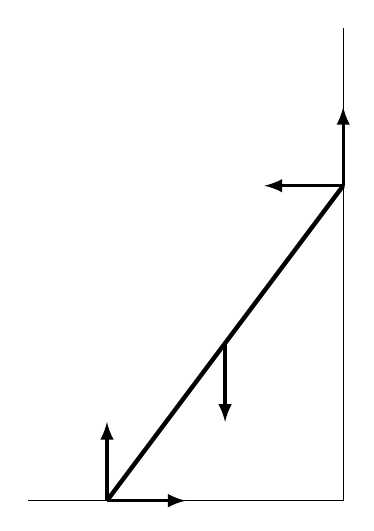
\begin{tikzpicture}

\draw (-4,0) -- (0,0) ;
\draw (0,0) -- (0,6) ;
\draw [ultra thick] (-3,0) -- (0,4) ;
\draw [very thick,-{latex}] (0,4) -- ++(0,1) ;
\draw [very thick,-{latex}] (0,4) -- ++(-1,0) ;
\draw [very thick,-{latex}] (-3,0) -- ++(0,1) ;
\draw [very thick,-{latex}] (-3,0) -- ++(1,0) ;
\draw [very thick,-{latex}] (-1.5,2) -- ++(0,-1) ; 

\end{tikzpicture}
\end{center}

\subsection*{ladder2}

\begin{center}
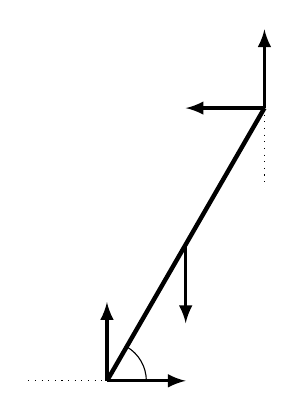
\begin{tikzpicture}
\draw [dotted] (-1,0) -- (1,0) ;
\draw [dotted] (60:4) -- ++(0,1) ;
\draw [dotted] (60:4) -- ++(0,-1) ;
\draw (0.5,0) arc [start angle = 0, end angle = 60, radius=0.5] ;
\draw [ultra thick] (0,0) -- ++(60:4) ;
\draw [very thick,-{latex}] (60:4) -- ++(0,1) ;
\draw [very thick,-{latex}] (60:4) -- ++(-1,0) ;
\draw [very thick,-{latex}] (0,0) -- ++(0,1) ;
\draw [very thick,-{latex}] (0,0) -- ++(1,0) ;
\draw [very thick,-{latex}] (60:2) -- ++(0,-1) ; 

\end{tikzpicture}
\end{center}

\subsection*{pendulum}

\begin{center}
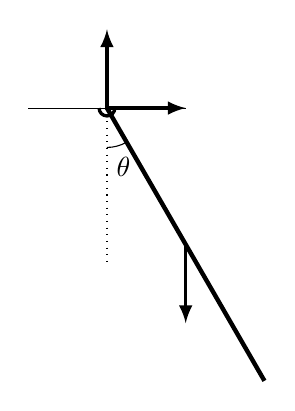
\begin{tikzpicture}

\draw (-1,0) -- (1,0) ;
\draw [very thick] (-0.1,0) arc  [start angle=-180,end angle=0,radius=0.1] ;
\draw [dotted] (0,0) -- (0,-2) ; 
\draw [ultra thick] (0,0) -- (-60:4) ;
\draw (0,-0.5) arc  [start angle=-90,end angle=-60,radius=0.5] ;
\draw (0,-0.5) node [anchor=north west] {$\theta$} ;
\draw [very thick,-{latex}] (-60:2) -- ++(0,-1) ;
\draw [very thick,-{latex}] (0,0) -- ++(0,1) ;
\draw [very thick,-{latex}] (0,0) -- ++(1,0) ; 

\end{tikzpicture}
\end{center}

\end{document}
